\documentclass[12pt, twoside, openany]{report}
\usepackage[dvips]{graphicx,color,rotating}
\usepackage{a4wide}
\usepackage[utf8]{inputenc}
\usepackage{enumerate}
\usepackage{verbatim}
\usepackage[polish,british]{babel}
\usepackage[T1]{fontenc}
\usepackage{geometry}
\geometry{left=25mm,right=25mm,%
bindingoffset=10mm, top=25mm, bottom=25mm}
\usepackage{latexsym}
\usepackage{amsthm}
\usepackage{palatino}
\usepackage{array}
\usepackage{pstricks}
\usepackage{textcomp}
\theoremstyle{definition}
\newcommand*{\norm}[1]{\left\Vert{#1}\right\Vert}
\newcommand*{\abs}[1]{\left\vert{#1}\right\vert}
\newcommand*{\om}{\omega}

\author{Paweł Paczuski}
\title{Tytuł pracy}

\begin{document}

% Zażółć gęślą jaźń.
\begin{titlepage}
\pagestyle{empty}

\noindent
\begin{Large}
\begin{table}[t]
\centering
\begin{tabular}[t]{lcr}
 
\includegraphics[width=70pt,height=70pt]{PW} & POLITECHNIKA WARSZAWSKA & \includegraphics[width=70pt,height=70pt]{ELKA}\\
& WYDZIAŁ ELEKTRONIKI & \\
& I TECHNIK INFORMACYJNYCH &
\end{tabular}
\end{table}

% \vfill
\begin{center}BACHELOR'S THESIS\end{center}
\begin{center}Computer Science\end{center}\end{Large}
% \vfill
\begin{center}
\Huge
\textbf{!!!DRAFT!!! Structured reporting system}
\end{center}
% \vfill\vfill
\vfill
\begin{center}
\Large
Author:\\
\LARGE
Paweł Paczuski
\end{center}
\vfill
\begin{center}
\Large
Thesis supervisor: Jan J. Mulawka PhD, DSc
\end{center}
\vfill
\begin{center}
\Large
Warsaw, June 2018
\end{center}
\newpage
\hfill
\begin{table}[b]
\centering
\begin{tabular}[t]{ccc}
............................................. & \hspace*{100pt} & .............................................\\
podpis promotora & \hspace*{100pt} & podpis autora
\end{tabular}
\end{table}


% \maketitle
\end{titlepage}
\thispagestyle{empty}
\newpage
\pagestyle{headings}
\setcounter{page}{1}
\hyphenation{Syl-ves-tra}
\hyphenation{Syl-ves-ter-a}
\begin{otherlanguage}{british}
\begin{abstract}
Structured radiological reporting system.

Design and implementation of a system that can be used by radiologists to create structured radiological reports. The system uses sets of standardized, frequently used phrases to: describe state of patient's body captured by other medical diagnostics methods, provide set of tools that minimize risk of mistake and increase productivity. 
\end{abstract}
\end{otherlanguage}

\begin{otherlanguage}{polish}
\begin{abstract}
streszczenie po polsku
\end{abstract}
\end{otherlanguage}

%-----------Początek części zasadniczej-----------
\tableofcontents
\clearpage







\chapter{Introduction}
\section{The need for medical diagnostics}
Everyday millions of physicians treat injuries and illnesses. Before a doctor can plan an individual treatment for a patient, they have to diagnose which organs are in pathological states\cite{bls}. This sometimes can be achieved by simply glancing at the body, however, there are many illnesses that require specialized set of tools and methods in order to observe which parts of patient's body are in an unwanted state. Through years of research, many different techniques were established and a separate specialization emerged -- radiology. Radiologists focus mainly on analyzing and interpreting diagnostic imagery and as a result of their work they create a document called radiological report which contains description of what can be observed in the image of patient body. Reports may contain description of state of particular organs, measurements (eg. radius, volume, concentration of certain substances in the blood), comparison of medical condition of a patient observed at different times and description of overall state of the patient. \\
\section{Existing solutions}
Currently, the research is focused on finding new ways of diagnosing diseases by  the use of more advanced equipment or brilliant algorithms that try to automate image analysis \cite{ai}. \\
On the other hand, there exist initiatives that try to improve quality of the radiological reports themselves. There are groups consisting of both computer scientists and physicians that try to standardize reports, prepare checklists that require doctors to describe patients' state in particular order and create a set of phrases that will be understood in the same way by all physicians \cite{snomed}. A lot of work has been done to provide common medical nomenclature for medical conditions, provide theoretical framework to describe relations between causes and effects of patients' condition. As there are more and more methods used to diagnose, the amount of information captured increases, so the reporting methodology has to be kept up to date with the state of art. This is why a very specific field -- structural reporting (SR) emerged. The basic idea is to provide a way to create radiological reports that convey as much semantics as possible in an easy to follow way. One can find great ideas implemented in such standards as SNOMED SR \cite{sr} and also HL7 version 3 Clinical Document Architecture (HL7 V3 CDA). By using these standards one can encode relations between organs and diseases (causality) in a very regular format. After encoding structure in the report, one can use algorithms to e.g. highlight what changed since last visit, look for diseases that were are diagnosed in the specified time range etc. This is very difficult to achieve when reports are stored in plain text. Structural reporting focuses on encoding only meaning -- the visual representation of resulting reports is a separate matter to discuss \cite{sr}.
In spite of the existence of these standards, it is almost impossible to find software that implements structural reporting techniques. One of the most important reasons is the fact that in order to understand benefits of SR, one has to acquire certain level of understanding of the typical workflow of a radiologist. 
\\ \\
\section{Definition of the engineering problem}
In this thesis I present a solution to the problem of not satisfactory productivity of radiologists by implementing a program used to create structured radiological reports. The system uses sets of standardized, frequently used phrases to: describe state of patient's body captured by other medical diagnostics methods, provide set of tools that minimize risk of mistake and allows radiologists to create reports faster.

\section{Typical workflow of a radiologist in Poland}
In order to find places where optimization of productivity could be applied, one has to get to know how a radiologist works and what are activities that waste significant amounts of time. \\
In a medium sized clinic, medical imagery is captured by a radiologic technologist who then uploads the data to the radiological information system (RIS) and attaches identification information to the images. This system distributes imagery to the team of radiologists that work for this clinic. 

Imagery can be distributed in one of the following manners:
\begin{itemize}
    \item particular patient is always serviced by the same radiologist or the RIS system 
    \item RIS system acts as an accumulator of images and radiologist decide which patient they focus on next
    \item certain types of medical examinations are are always assigned to a radiologist that is specialized in describing them
\end{itemize}

After receiving diagnostic imagery, a radiologist uses special software called viewer\cite{viewer} to navigate through images, make measurements by using visual tools like virtual ruler and examine what is the state of patient's body. In parallel to this, the doctor uses text editor and describes what he or she sees in the images. 
\begin{figure}
    \centering
    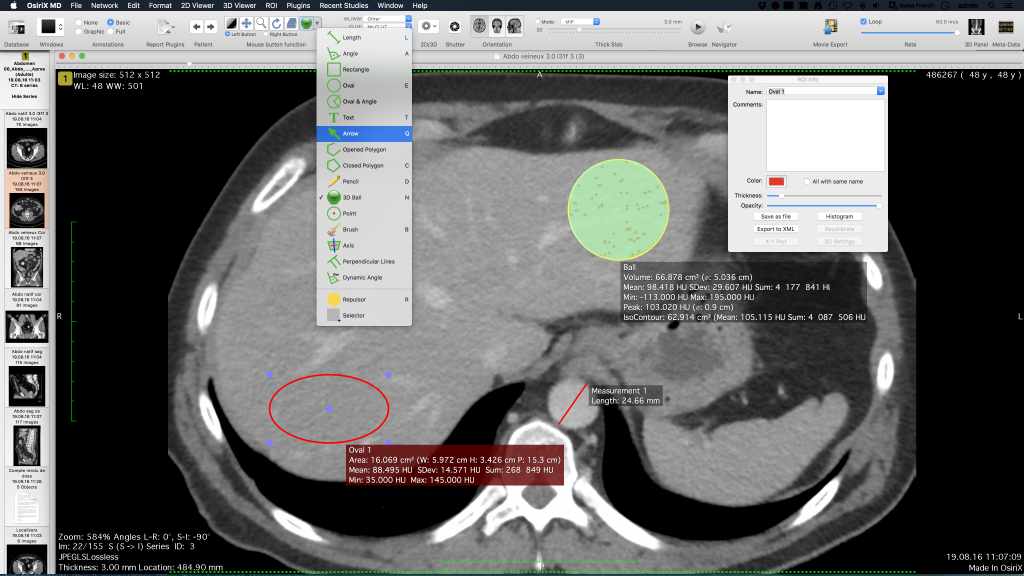
\includegraphics[width=0.9\linewidth]{osirix}
    \caption{OsiriX is one of the most popular image viewers used by the radiologists}
    \label{fig:osirix}
\end{figure}



\section{Discussion about presented workflow}
\subsection{The good parts}
\subsubsection{Viewer software provides expected functionality}
Viewer software has a very stable position on the market and is perfectly tailored to the needs of a radiologist. It often uses advanced techniques of 3D graphics to present patient's body as accurately as possible.
\subsubsection{RIS systems make it easy to exchange data between physians}
There is no need need for the radiologist to deliver the radiological report to the other physician personally as it is done automatically. Also, RIS systems provide good means of distributing diagnostic imagery to radiologists.
\subsection{The bad parts}
\subsubsection{Focus on text rather than semantics}
It is expected that the radiologist will produce a consistent, ordered report by means of text editors. Some RIS systems provide basic text formatting functionality like italicization, underlining but they are very limited to the textual presentation of the report. There are no means to encode relations in this representation.
\subsubsection{Each radiologist has their own style of writing}
Usually there are no structural expectations about the resulting report. Each radiologist can have their own style of writing, order of organs and observation. This leads to the waste of time as people who read the report have to make some effort to infer the meaning. 
\subsubsection{Selective description}
It is very frequent that radiologists include in the report only things that they consider bad for the patient. This makes the report more goal-oriented but it means that it is useless to get to know the overall state of patient body.
\subsubsection{Copy-paste}
Radiologists try to solve the problem of typing on their own by crating templates that contain certain pathologies listed and what they do is execution of the commonly called 'copy-paste' method to create report content. Sometimes they do not notice parts of copied text that are different from the actual state of the body, so the reports may contain observations that are false. 

\section{Other ways to create radiological reports}
In many English-speaking countries the workflow of a radiologist differs in the way the radiological report is generated. A radiologist may record their voice while describing the imagery vocally. The recordings are then transcribed using either speech recognition algorithms or manually by technologists. Having a good skill of typing by a radiologist is not required, only knowledge to interpret imagery is used. This approach, however, has some architectural disadvantages. More personnel is needed -- technologists, who transcribe the recorded voice\cite{speech-impact}. Also, it is difficult to make changes to what has been said. In some cases, a mistake can made while transcribing the text \cite{speech-africa}.

\section{Problem definition}

After analyzing bad parts of the presented workflow and general situation on the market -- demand for radiological services increases but the number of radiologists appears to be constant, the author decided to design and implement a system that would be used by radiologists to encode semantics of diagnostic imagery in a form that can be easily transformed to the human readable form, analyzed by algorithms. 









\chapter{Description of the proposed solution}
\section{General idea}
\subsection{Area of interest}
The system that is proposed in this thesis focuses entirely on the part of the typical radiological workflow in which a radiologist focuses on the textual description of what can be seen in the diagnostic imagery.
\subsection{Contextual suggestions}
The author analyzed several hundreds of anonymized radiological reports and observed that a lot of time could be saved, if a radiologist would at any time select text fragments from a predefined set of possibilities that are appropriate to the current context. This approach can be seen in the way Integrated Development Environment (IDE) for statically typed languages (e.g. Visual Studio supporting C\#) are suggesting what the programmer can write based on the namespace, class, scope they currently edit.

In the case of programming language the problem is defined in a more strict way. They are very often supported by definitions of formal grammars \cite{csharp-spec}. Radiological reports, however, are creating using  natural language, so there always exist some exceptions.

\section{Workflow of a radilogist who uses the proposed system}
In figure \ref{fig:report-workflow} a typical workflow of a radiologist is represented in the form of a flowchart. 
\begin{figure}
    \centering
    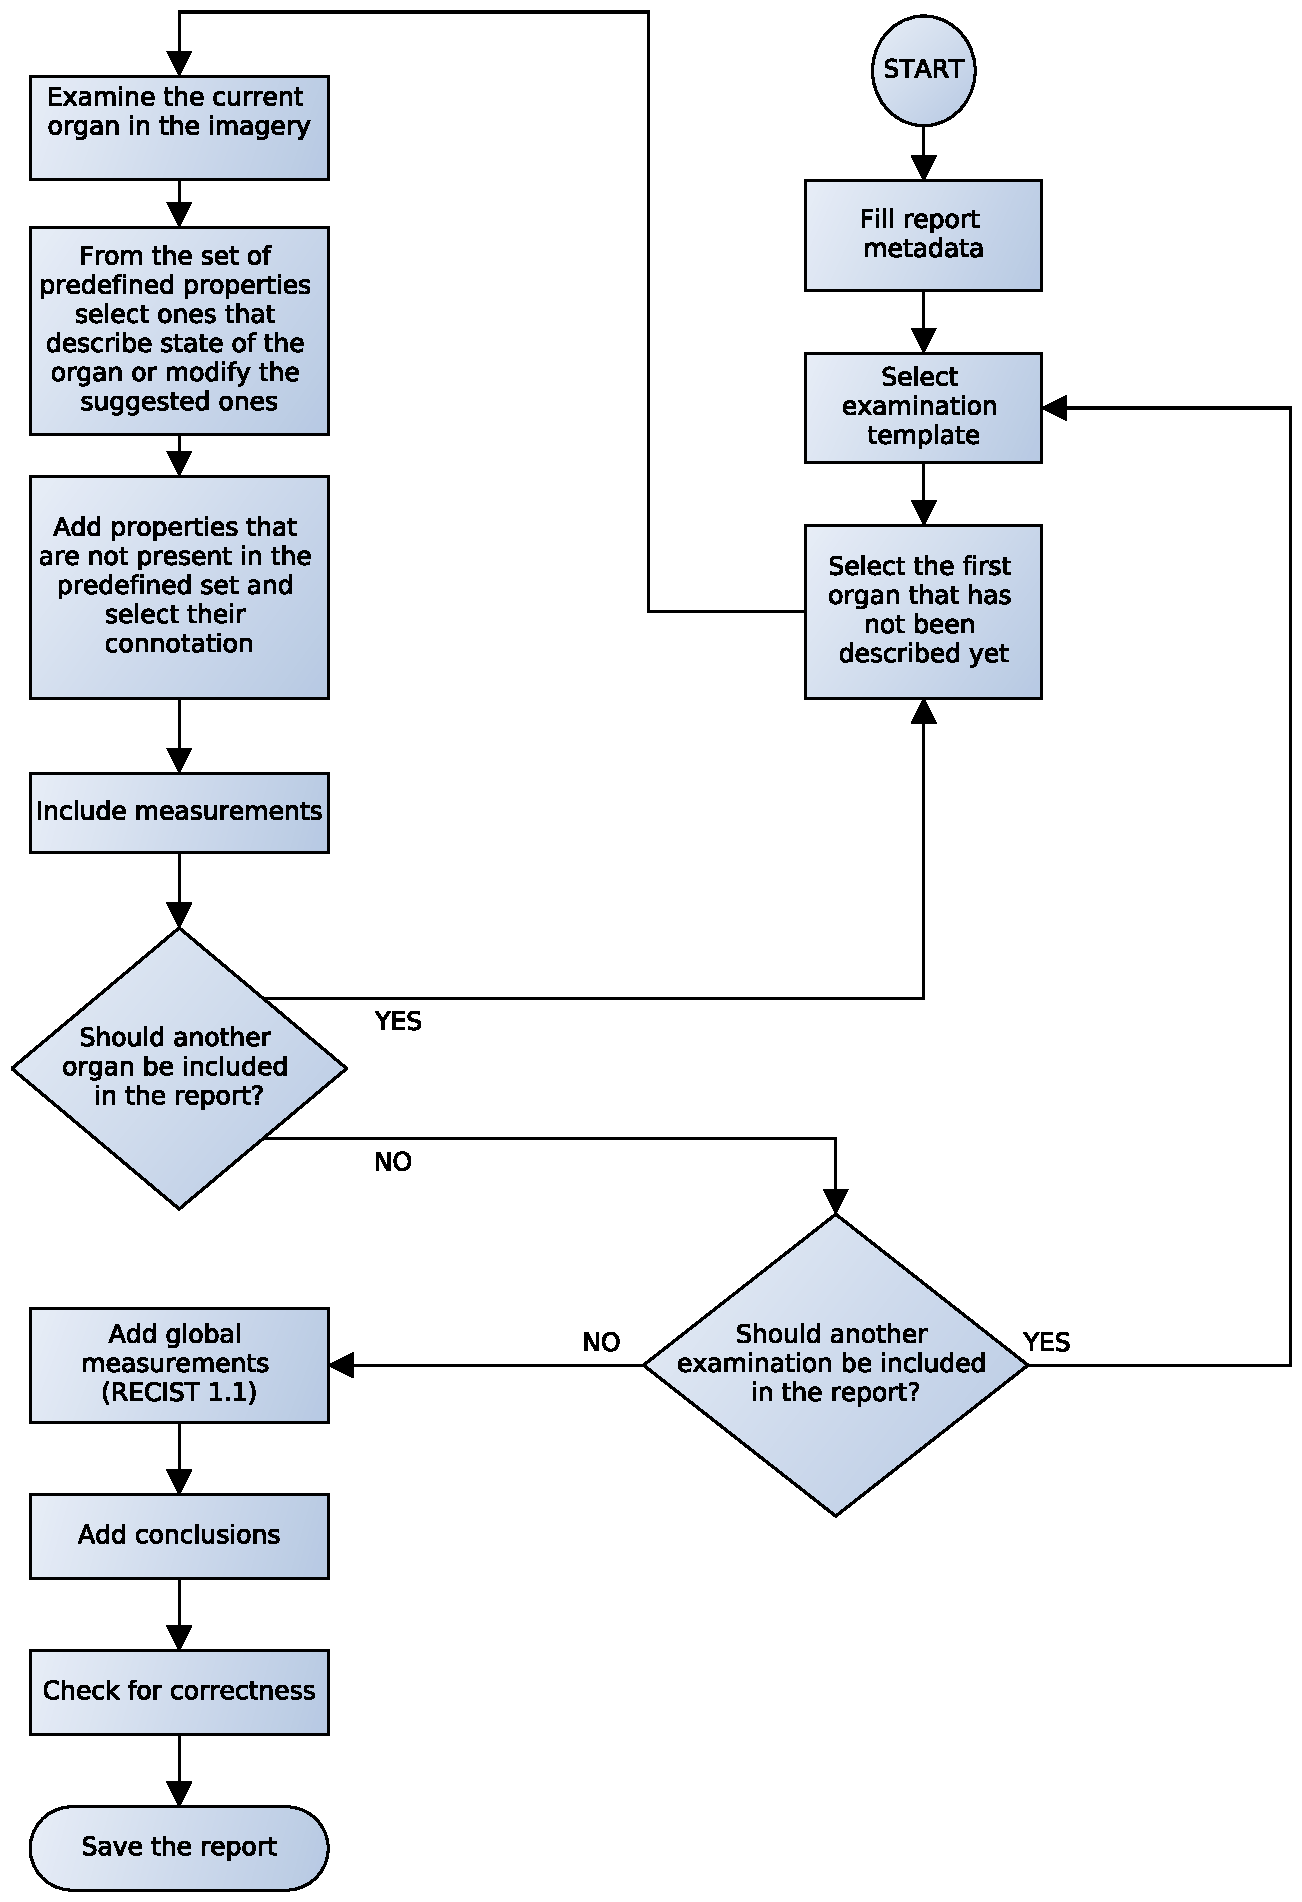
\includegraphics[width=\linewidth]{report-workflow.pdf}
    \caption{Workflow of a radiologist who uses the proposed system to create contents of a radiological report.
        \label{fig:report-workflow}
    }
\end{figure}
\section{Proposed reporting ontology based on ideas from DICOM SR and HL7 CDA}
In order to provide context for the radiologist at any given moment, it is proposed to split report into the following nested structures:
\begin{enumerate}
    \item Examinations -- single report may have many of them
    \item Organs -- single examination may have many of them
    \item Properties -- single organ may have many of them
\end{enumerate}
Figure \ref{fig:report-semantic} shows how report structures relate by semantic relations.
\begin{figure}
    \centering
    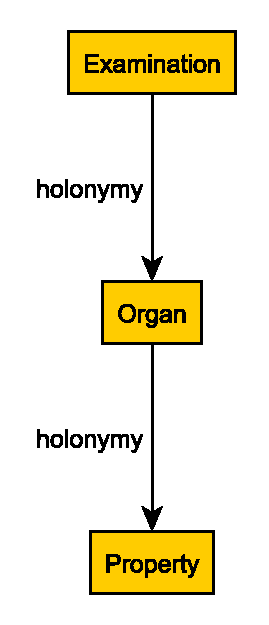
\includegraphics{report-semantic.pdf}
    \caption{Structure of a radiological report created \label{fig:report-semantic}}
\end{figure}

\begin{figure}
    \centering
    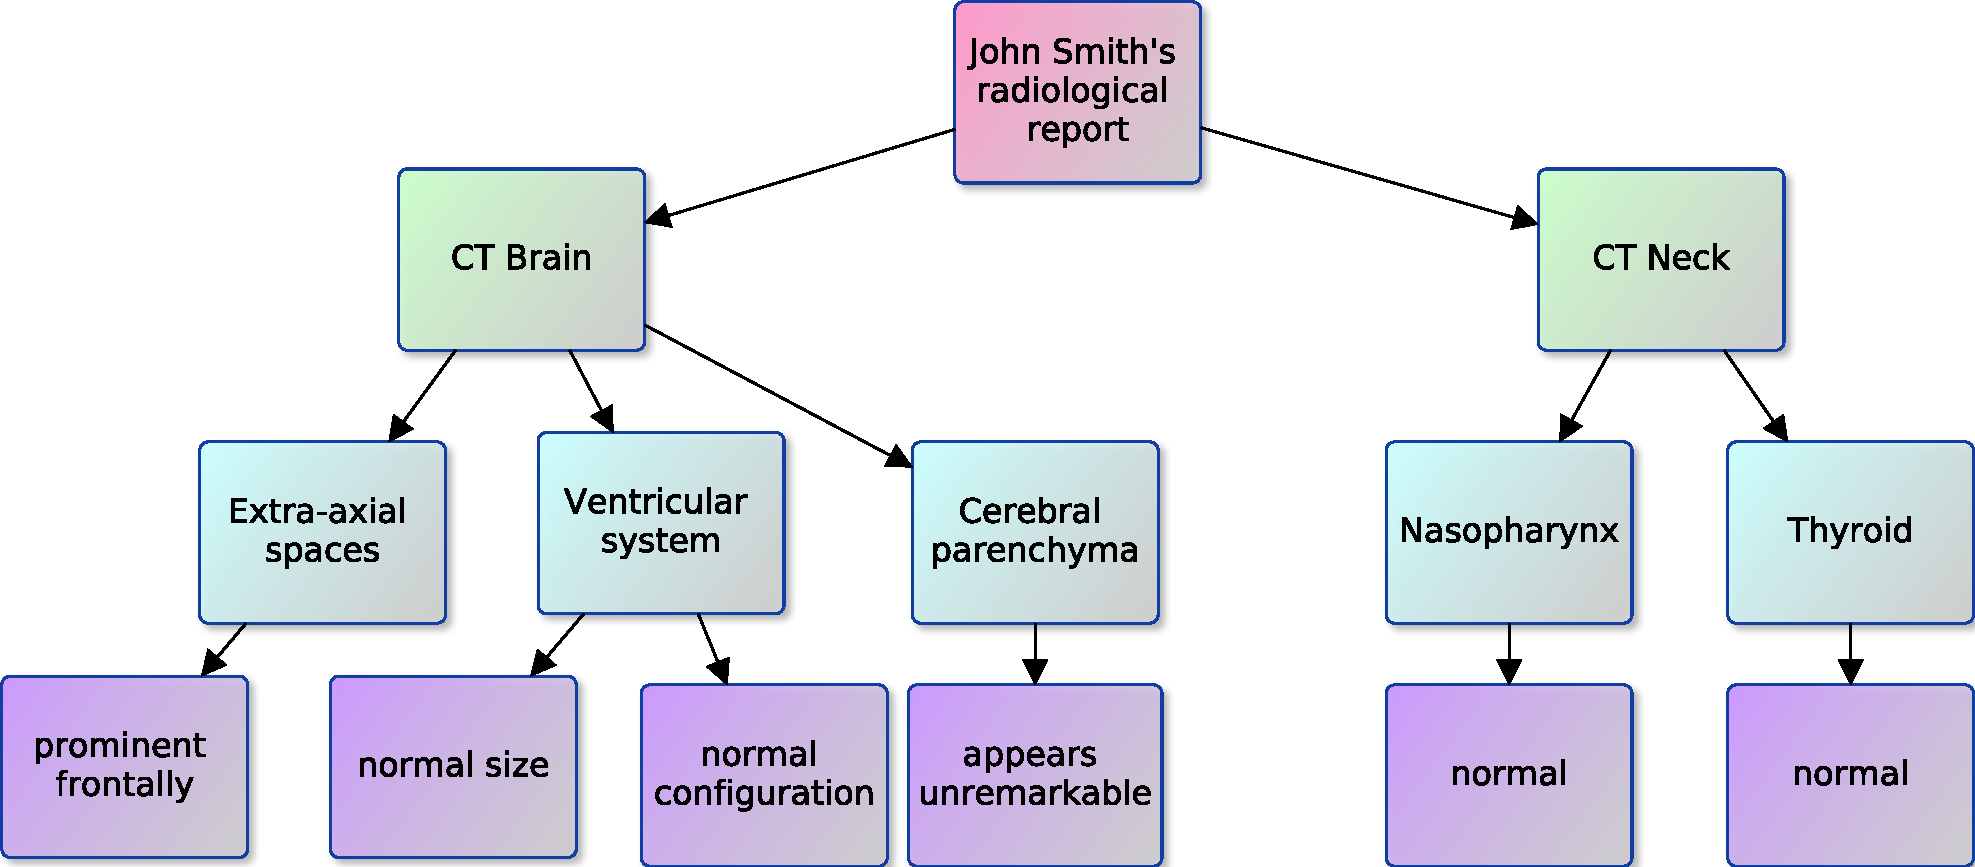
\includegraphics[width=\linewidth]{report-tree.pdf}
    \caption{Structure of a radiological report created \label{fig:report-tree} using proposed system. For simplicity, only names of nodes are presented (associated metadata were omitted)}
\end{figure}

By using this ontology, a radiologist can create a report that is similar in structure to a tree (as it is presented in figure \ref{fig:report-tree}). At any given moment, the doctor modifies the tree at a single level, which allows for suggesting what are the items that can be included. The idea was taken from statically typed languages which thanks to their strictness allow for coding with smaller number of mistakes at the lexical level \cite{static-lang}.

\subsection{Connotation}
Moreover, each property has a semantical attribute called connotation. Connotation is used to highlight the impact of this property on the result of the organ and examination. This attribute can have one of three values: positive, negative and neutral. 
\subsection{Metadata}
Report may also contain some metadata which can be used identify the patient whose body is described in it. Shape of these pieces of information strongly depends on the RIS system used in a clinic. These data have no special influence on the semantics of report so it has no detailed description in this work.

Names for these ontological structures were chosen so it is easier for radiologists to imagine what they describe, however, they can be used not strictly (e.g. in CT scan as an organ one may include details about intracranial hemorrhage which is a kind of bleeding within the skull \cite{ich} but not an organ in its very meaning)

\section{Examination template}
Examination template (or simply 'template') consists of an ordered list of all organs that could be described with all and some portion of metadata used for filtering like category, discipline. Each organ in a template has an ordered list of all properties that can describe it. Every property can have connotation predefined. 

\begin{figure}
    \centering
    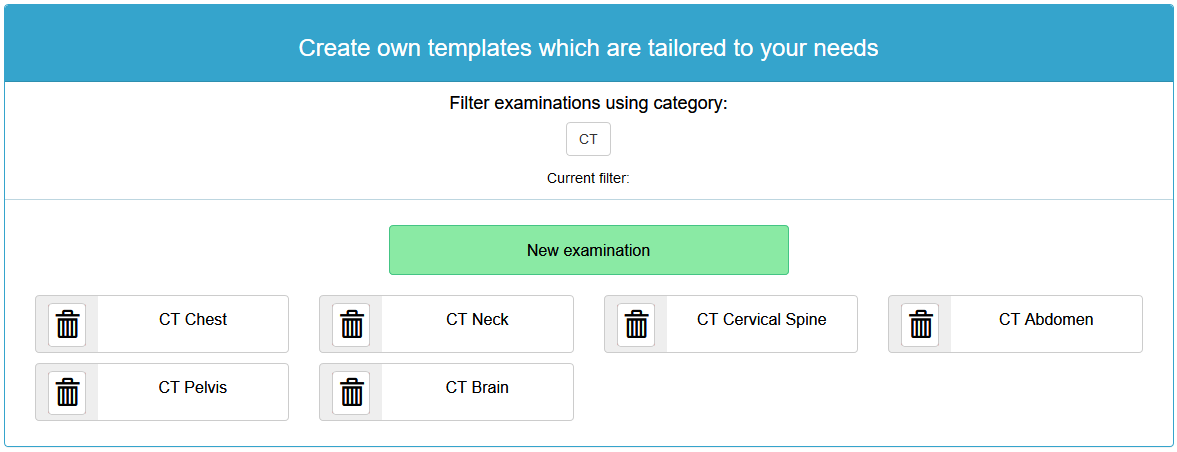
\includegraphics[width=0.9\linewidth]{templates-list.PNG}
    \caption{List of templates that can be edited by the user\label{fig:templates-list}}
\end{figure}
\begin{figure}
    \centering
    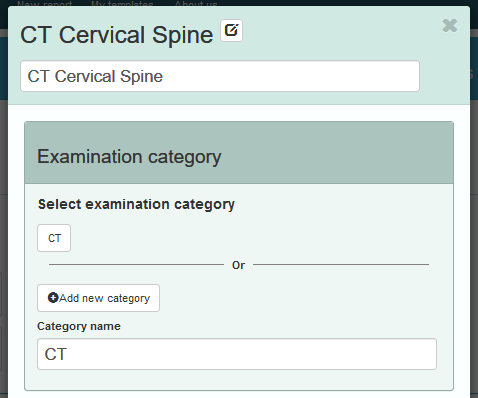
\includegraphics{template-metadata.PNG}
    \caption{GUI used to edit template metadata \label{fig:template-metadata}}
\end{figure}
\begin{figure}
    \centering
    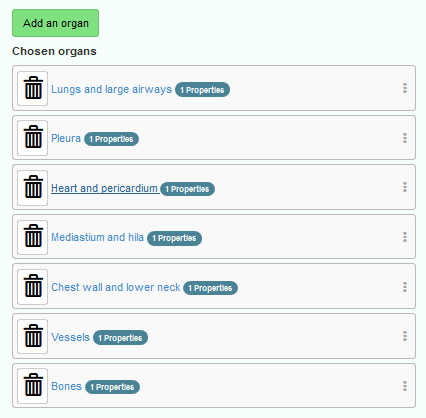
\includegraphics{template-organs-list.PNG}
    \caption{GUI used to edit organs \label{fig:template-organs-list}}
\end{figure}
\begin{figure}
    \centering
    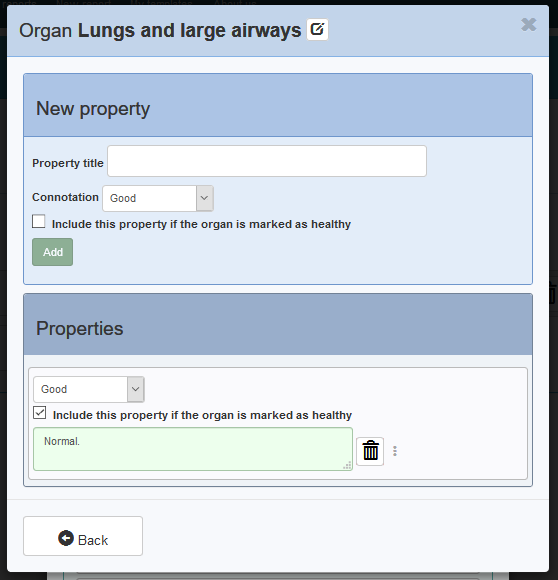
\includegraphics{template-property-list.PNG}
    \caption{GUI used to edit properties of an organ. User can predefine connotation and tell the program that this property can be automatically included if the organ is marked as healthy \label{fig:template-property-list}}
\end{figure}

Examination templates can be prepared by the leader of radiologists team, so the team can use common language to describe diagnostic imagery. Templates prepared by the leader constitute the so called set of public examinations.

If a given template is not sufficient for a particular radiologist, they can  create their own template from scratch or extend the existing one (an action that for some people can resemble forking a repo in git \cite{forking})


\section{Assumptions}
After observation of actions taken by radiologists while working in environments like hospital, medium-sized clinic, independent teleradiological practice the following assumptions are suggested:
\begin{itemize}
    \item Radiologists prefer using mouse to keyboard
    \item The user interface of the program should be simple 
    \item Reports must be rendered in a way that allows for copying using clipboard as radiologists developed custom ways to save drafts of reports.
    \item The system should allow for exporting reports into formatted text and pdf
    \item Text formatting should be based on semantics that is encoded by a radiologist.
    \item The system should favor reports that describe the whole state of body, not only organs in bad condition.
    \item The system should allow to automatically include in the report segments of text that are (almost) always used (sometimes due to some legal regulations).

\end{itemize}
\section{Goals}
\begin{itemize}
\item Minimize the time radiologist uses keyboard
\item Split report into structural parts that allow to express description of patient's state.
\item Any fragment of templated text should be editable. 
\item Maximize number of reports that can be generated by a radiologist in a unit of time.
\item At any time allow to include
\end{itemize}


\section{Productivity improvements}
\subsection{Using templates}
The goal to increase productivity of a radiologist is achieved mostly by decreasing the average time a doctor types on keyboard. By the usage of examination templates, the time spent to create the schema of the report is shifted from the doctor to the leader of the radiologists team. It can take a lot of time to create a template that is both universal and correct but it is a one-time-only investment. The more templates are created using a template, the more it pays off in the long run.

\subsection{Mark organ as healthy}
In the proposed system, each property has additional attribute (it can be set in template editor) named "include if organ healthy". When a radiologist creates a report, an organ can be marked as healthy, which means that all properties that have this attribute set to true are automatically included in the report. This allows to quickly add properties that are very commonly used. 
In order to minimize the possibility of inclusion a  property that does not correspond to the actual state of patient's body, only properties with positive connotation can have this attribute set. 

\subsection{Calculators}
There exist many standardized numerical methods used to asses whether values of certain parameters are in the range suggesting poor health condition, e.g. one of the most popular parameter is the body-mass-index (BMI) which is calculated using formula:
\begin{equation}
BMI=\frac{mass}{height^2}
\end{equation} 
After calculating this index, a radiologist has to look through tables to check whether the value is usually attached to people with obesity or not. 
BMI is one example of hundreds techniques used by doctors. It is not integrated, however, within the proposed system.

\subsubsection{RECIST 1.1}
During the design of the proposed systems several radiologists who specialize in oncological medicine reporting suggested that a method called  Response Evaluation Criteria In Solid Tumors (RECIST 1.1) is of special importance to them. This method is used to assess whether tumors in cancer patients improve, stay the same, or worsen during treatment \cite{wiki-recist}. As there are hundreds of similar methods used by radiologists, it would be impossible to implement them in the proposed system all at once, so it was decided to use RECIST 1.1 as a proof of the concept of calculators that can be used in structured reports.
A radiologist, while creating a report, can measure size of lesions and write down the results of measurement in the report. Proposed program should recognize that the numerical value represents a measurement and should suggest whether it should be included in the calculation of RECIST 1.1 or not.

\section{Reporting quality improvements}
\subsection{Standardized nomenclature}
There exist several attempts to standardize the language doctors use to describe precisely medical imagery. Templates created for the proposed structured reporting system can be created with the help of terminologists who specialize in systematized nomenclatures like SNOMED and LOINC to create reports what can lead to improved reporting quality as a radiologist does not have to explore huge volumes of precise textual definitions of terms used. 
\subsection{No repetitions}
Templates can be interpreted as TODO-lists containing tasks which have to be done while describing medical imagery, so a radiologist can be sure that nothing was omitted or no item appears twice in the report as a result of a mistake.
\subsection{Reports have ordered list of elements}
Reports created using the proposed system can be represented as trees, nested lists of items, so it is easy to spot relationships between properties and organs and also differences between two reports describing one patient.
\subsection{Highlighting the most important pieces of information}
The most important pieces of information can be highlighted using proper value of connotation. When one of properties of an organ should be interpreted as a main cause of health problems it is marked as a pathology. When the report is then rendered as a document, this property can have e.g. different font color, some text-decoration element or different background color.
\subsection{Shift from difference reporting to the current state reporting}
There exists practices quite popular among radiologists mostly from smaller clinics that are considered as bad among professionals. One is to include in the radiological report only properties of body which they consider as bad for patient's health. Due to the subjective nature of the report there were cases when a radiologist skipped a finding that was important stating the patient was healthy leading to more difficult and expensive treatment later.
There were also cases when a radiologist was unable to compare current state with descriptions of several images that were taken at different times, only with the last one. The doctor stated that there is a progress in treatment, but in comparison to the second from the last description, the health condition worsened. \cite{risk-management}
Templates created using the proposed system can favor radiological reports that are more self-contained -- they describe both bad and good properties of patient's state.

\subsection{Possibility of automated comparison}


\section{Integration with existing systems}
As there are many ways to store radiological reports. Many radiologists work remotely for several companies that have different RIS systems. It is very difficult to integrate the system with all of the systems as it requires cooperation of both developer of the proposed system and the developers of the RIS system. 

The approach taken by the author is very robust, works for all of the systems used nowadays but is not very elegant from the point of view of software engineering. 
After generating the report using the proposed system, it is the radiologist's duty to manually copy the resulting report to the RIS system. It is simplified in a way that the report is automatically copied to the clipboard after clicking on its content.

On the other hand, the proposed system was designed in a way that makes it easy to create communication channels that can be used to integrate this system with existing RIS systems. 

\section{Evolutionary approach to software development}







\chapter{Implementation of structured reporting system}

\section{Technological stack}
\section{Templates}
\section{New Report}
\section{Report history}
\section{Comparing reports}






\chapter{Validation of the proposed solution and examples of places where it was used}
\section{Teleradiologists}

\section{Hospital}

\section{Large network of clinics}

\chapter{Ideas for the future}
\chapter{Conclusion}

\chapter {Appendices}
\section{How to setup the program}
\section {How to use the program}


%-----------Koniec części zasadniczej-----------

\begin{thebibliography}{11}
\bibitem{bls} https://www.bls.gov/ooh/healthcare/physicians-and-surgeons.htm, accessed 08.10.2017 13:30
\bibitem{ai} M. Recht, N. Bryan, Artificial Intelligence: Threat or Boon to Radiologists?

N1  - doi: 10.1016/j.jacr.2017.07.007
\bibitem{snomed} T. Benson, Principles of health interoperability HL7 and SNOMED.
\bibitem{sr} D. A. Clunie, DICOM Structured Reporting
\bibitem{hl7cda} http://www.hl7.org/Special/committees/structure/index.cfm 
\bibitem{techonologist} https://www.asrt.org/main/careers/careers-in-radiologic-technology/who-are-radiologic-technologists
\bibitem{workflow} https://radiologystories.com/2013/10/31/the-typical-radiologist-work-day/
\bibitem{viewer}
http://www.osirix-viewer.com/osirix/overview/
\bibitem{speech-impact}
S. Langer, Impact of Speech Recognition on Radiologist Productivity
\bibitem{speech-africa} J. du Toit, R. Hattingh and R. Pitcher, The accuracy of radiology speech recognition
reports in a multilingual South African teaching hospital.
\bibitem{csharp-spec}
https://docs.microsoft.com/en-us/dotnet/csharp/language-reference/language-specification/lexical-structure
\bibitem{ich} http://emedicine.medscape.com/article/1163977-overview
\bibitem{static-lang}
    S. Hanenberg, S. Kleinschmager, R. Robbes, É. Tanter, A. Stefik, An empirical study on the impact of static typing on software maintainability
\bibitem {forking} https://help.github.com/articles/fork-a-repo/
\bibitem{wiki-recist} 
https://en.wikipedia.org/wiki/Response\_Evaluation\_Criteria\_in\_Solid\_Tumors
\bibitem{risk-management} https://www.ncbi.nlm.nih.gov/pubmed/3497558
\end{thebibliography}
\clearpage
\begin{otherlanguage}{polish}
\pagestyle{empty}
\noindent Warszawa, dnia ...............
\vspace{5cm}
\begin{center}
\LARGE{Oświadczenie}
\end{center}
Oświadczam, że pracę inżynierską pod tytułem: ,,Tytuł pracy'', której promotorem jest prof. dr hab. Jan Wybitny, wykonałem/am samodzielnie, co poświadczam własnoręcznym podpisem.
\vspace{2cm}
\begin{flushright}
...........................................
\end{flushright}
\end{otherlanguage}
\end{document}